\subsection{Functional Requirements}


\begin{figure}[!htb]
\subsubsection{Class Diagram}
\centering
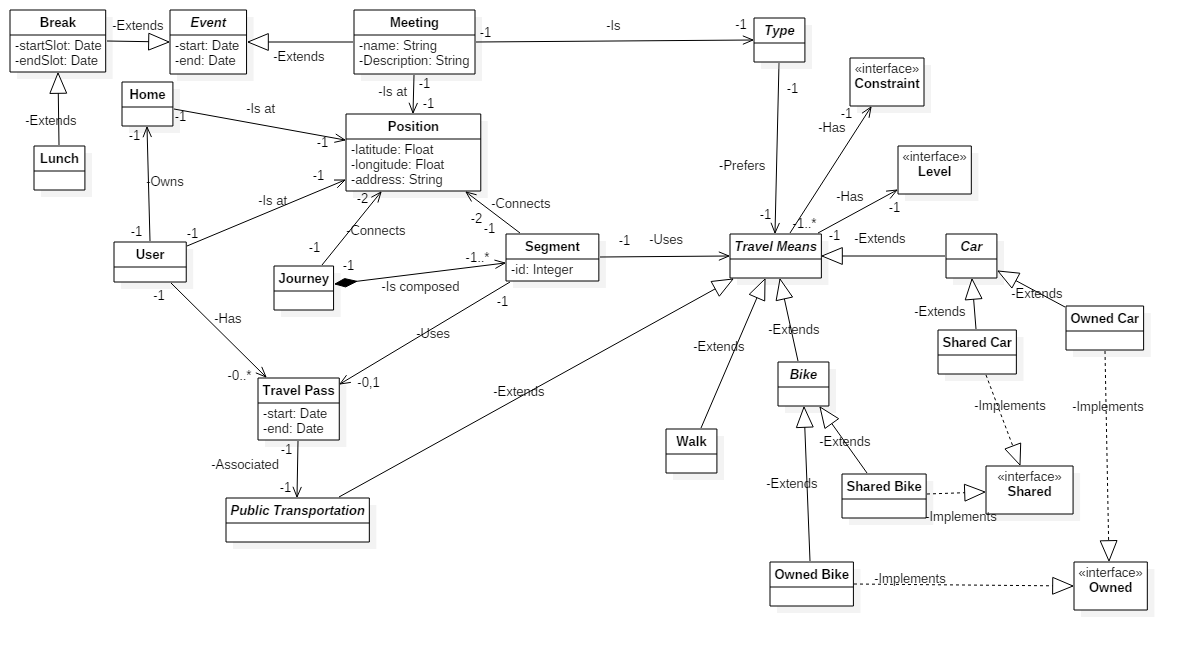
\includegraphics[scale=0.4]{images/ClassDiagram}
\caption{Class diagram}
\label{ref:classdiagram}
\end{figure}

\begin{figure}[!htb]
\subsubsection{Use Case Diagram}
\centering
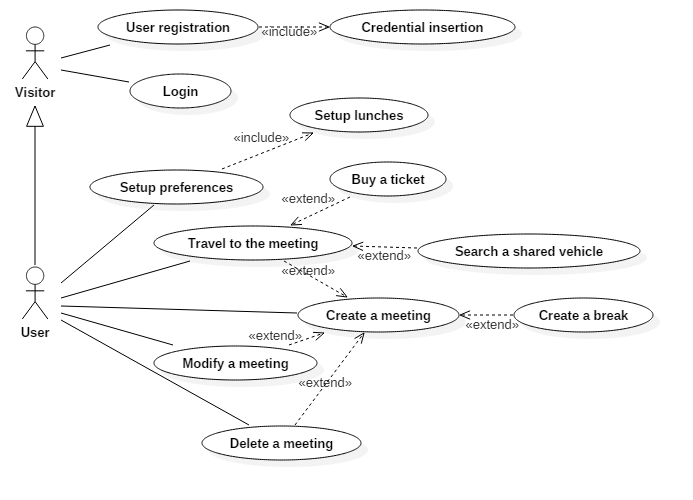
\includegraphics[scale=0.6]{images/UseCaseDiagram}
\caption{Use case diagram}
\label{ref:classdiagram}
\end{figure}
\clearpage
\subsubsection{Use Case Descriptions}

In this section are listed some common or significant use cases derivable from
the Use Case diagram.

%Visitor's registration%
\begin{tabular} { p{5cm} p{8cm} } 
\textbf{Visitor's registration} & \\
\hline
\textbf{Actor:} & Visitor \\ 
\textbf{Goals:} & G.1 \\ 
\textbf{Input conditions:} & The visitor is on the home page. \\
\textbf{Event flow:} & \begin{enumerate}
						\item
						The visitor clicks any button and is redirected to the login page.
						\item
						The visitor clicks on the “Sign Up” button to start the registration process.
						\item
						The visitor fills all the mandatory fields.
						\item
						The visitor clicks on the “Sign Up“ button.
						\item
						The system send the data to the server.
						\item
						The system sends a confirmation email to the new user.
						\end{enumerate}\\ 
\textbf{Output conditions:} & The visitor successfully ends the registration process and is redirected to the home page. From now he can login to the application and start using that. \\ 
\textbf{Exception:} & \begin{enumerate}
						\item
						The visitor is already an user.
						\item
						The visitor inserts not valid information in one or more mandatory fields.
						\item
						The visitor chooses an email that has been associated with another user.
					\end{enumerate}
All exceptions are handled notifying the issue to the visitor and taking back the Event Flow to the point 2. \\
\hline
\end{tabular}


%User's login%
\begin{tabular} { p{5cm} p{8cm} } 
\textbf{User's login} & \\
\hline
\textbf{Actor:} & User \\ 
\textbf{Goals:} & G.1 \\ 
\textbf{Input conditions:} & The visitor is on the login page. \\
\textbf{Event flow:} & \begin{enumerate}
				\item
				The user inserts his credentials into the “email” and “password” fields.
				\item
				The user clicks on the “Login” button in order to access.
			\end{enumerate} \\ 
\textbf{Output conditions:} & The user is successfully redirected to the
home page.\\ 
\textbf{Exception:} & \begin{enumerate}
				\item
				The user inserts a not valid email.
				\item
				The user inserts a not valid password.
			\end{enumerate}
All exceptions are handled notifying the issue to the user and taking back the Event Flow to the point 1. \\
\hline
\end{tabular}


%User creates a meeting%
\begin{tabular} { p{5cm} p{8cm} }  
\textbf{Create a meeting.}\\
\hline
\textbf{Actor:} & User \\ 
\textbf{Goals:} & G.2, G.3 \\ 
\textbf{Input conditions:} & The user is already logged into the system and is into the schedule page. \\
\textbf{Event flow:} & \begin{enumerate}
				\item
				The user clicks on the “New meeting” button to start the creation process.
				\item
				The user inserts the information  into the fields and the type.
				\item
				The user clicks on the “Create meeting” button.
			\end{enumerate}\\ 
\textbf{Output conditions:} & The user is successfully redirected to the
meeting.\\ 
\textbf{Exception:} & \begin{enumerate}
				\item
				The name isn’t valid.
				\item
				The start hour doesn’t precede the end hour.
				\item
				The start hour and end hour precede the current date.
				\item
				Exists an another meeting with the same hours. 
			\end{enumerate}
All exceptions are handled notifying the issue to the user and taking back the Event Flow to the point 2.
\\
\hline
\end{tabular}


%User travels to the meeting%
\begin{tabular} { p{5cm} p{8cm} }  
\textbf{Travel to the meeting}\\
\hline
\textbf{Actor:} & User \\ 
\textbf{Goals:} & G.4, G.8 \\ 
\textbf{Input conditions:} & The user is already logged into the system and is into the schedule page. \\
\textbf{Event flow:} & \begin{enumerate}
				\item
				The user clicks on the desired meeting and is redirected into the meeting information.
				\item
				The user clicks on “Navigate” and goes into navigate page.
				\item
				The navigate page helps the user with indications.
				\item
				When the user is arrived at the desired location, the application notify him.
			\end{enumerate} \\ 
\textbf{Output conditions:} & The user is successfully redirected to the
schedule.\\ 
\textbf{Exception:} & \begin{enumerate}
				\item
				The GPS is unavailable.
				\item
				The location isn’t found. 
			\end{enumerate}
All exceptions are handled notifying the issue to the user and taking back the Event Flow to the point 1. \\
\hline
\end{tabular}


%User selects preferences and filters options%
\begin{tabular} { p{5cm} p{8cm} }
\textbf{Setup preferences} \\
\hline
\textbf{Actor:} & User \\ 
\textbf{Goals:} & G.5, G.7 \\ 
\textbf{Input conditions:} & The user is already logged into the system and is into the home page. \\
\textbf{Event flow:} & \begin{enumerate}
				\item
				The user clicks on “Setting” button and is redirected into setting page.
				\item
				The user inserts his preferences about travel means and lunch timetable.
				\item
				The user confirms the new information with “Confirm” button.
			\end{enumerate}\\ 
\textbf{Output conditions:} & The user stays in the setting page.\\ 
\textbf{Exception:} & \begin{enumerate}
				\item
				The user doesn’t insert numbers in the lunch fields.
			\end{enumerate}
All exceptions are handled notifying the issue to the user and taking back the Event Flow to the point 2. \\
\hline
\end{tabular}


\subsubsection{Sequence Diagrams}
